\section{System Overview}
\label{sec:system}
\textsc{Synopsis} is implemented on top of the \textsc{Neptune} stream processing system \cite{buddhika2016neptune} as a specialized layer for geospatial data.
In this section, we will briefly introduce Neptune followed by a discussion on the design of \textsc{Synopsis}.

\subsection{Neptune}
Neptune is a distributed stream processing system which is optimized to process high throughput data streams.
It is designed to cope with application requirements such as high volumes of small stream packets, high and variable data rates and heterogeneity within stream processing jobs.
Satisfying these requirements imposes various system level challenges including possible buffer overflow errors, increased number of context switches, object creation overhead and memory management issues.
Neptune takes a holistic approach that considers CPU, memory, network and kernel issues to address these challenges.
This is achieved through optimizations such as application level buffering, batched scheduling, object reuse, built-in support for backpressure and selective compression to ensure better utilization of system resources.

Users can deploy stream processing jobs as directed acyclic graphs in Neptune.
A stream processing graph consists of a set of stream ingestion points and stream processors (vertices) and streams connecting these operators (edges).
To provide each job with a initial load-balanced deployment plan to start with, each operator in a stream processing graph can be annotated with a parallelism level while each stream can be associated with a partitioning scheme.

\subsection{\textsc{Synopsis}}
\textsc{Synopsis} is a distributed sketch constructed over voluminous data streams.
The number of nodes (or sketchlets) that comprise the sketch varies dynamically as the sketch upscales or downscales to cope with data arrival rates and memory pressure.
Each sketchlet is responsible for one of more geographical scopes and is implemented as a stateful Neptune stream processor that can build and retain state over time.
A stream partitioning scheme, based on the Geohash algorithm (described in Section 3.2), is used to route packets to the appropriate sketchlet.
Sketchlets ingest stream packets and construct compact, in-memory representations of the observational data by extracting metadata from individual stream packets.
During upscaling and downscaling operations, the geographical extents managed by a sketch varies.

Each sketchlet instance extends Neptune's generic stream processor to provide auxiliary services that are needed to construct, update and maintain the sketch and also to adapt to changing system conditions.
These services are control plane, gossip subsystem and querying subsystem as depicted in Figure~\ref{fig:rivulet-archi}.
%
\begin{figure}
    \centerline{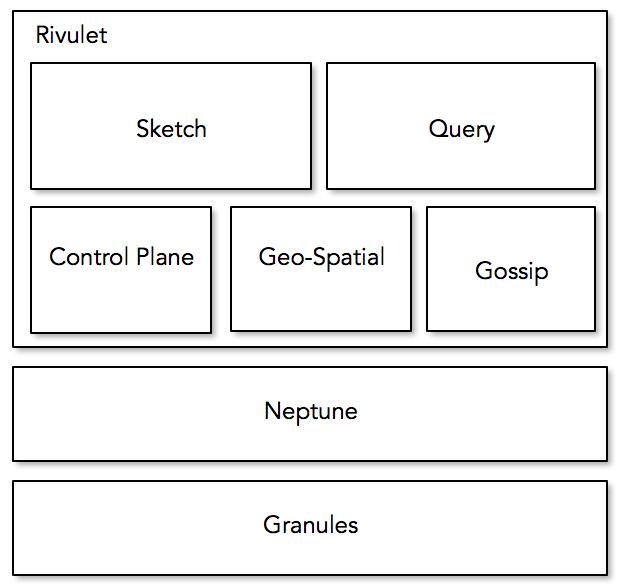
\includegraphics[scale=0.5]{figures/rivulet-archi.png}}
    \caption{\textsc{Synopsis} is implemented as a specialized layer for geo-spatial data on top of Neptune stream processing system.}
    \label{fig:rivulet-archi}
\end{figure}
%
\begin{description}[leftmargin=*]
	\item[Control plane:] The control plane is responsible for orchestrating control messages exchanged between \textsc{Synopsis} nodes as part of various distributed protocols such dynamic scaling.
    The control plane is decoupled from the data plane to ensure higher priority and low latency processing without being affected by buffering delays and backpressure during stream processing.

	\item[Gossip subsystem:] While a majority of the \textsc{Synopsis} functionality relies on the local state (or knowledge) constructed at a particular node, certain functionalities require an approximate global knowledge.
    For instance, each sketchlet maintains a Geohash prefix tree to assist in distributed query evaluations by forwarding queries to sketchlets that are responsible for particular geographical extents.
    In order to establish and maintain this global view of the entire system, sketchlets gossip about their state periodically as well as when there is a change in the state which nodes comprising the sketch are interested in.
    Sketchlets gossip state information periodically (based on combination of time intervals and the number of pending updates).
    \textsc{Synopsis} supports eventual consistency with respect to these updates given that there is an inherent propagation and convergence delay in such gossips.

	\item[Querying subsystem:] The querying subsystem is responsible for distributed evaluation of queries.
    This involves forwarding queries to relevant sketchlets; in some cases, multiple sketchlets may be involved based on the geographical scope of the query.

    \item[Monitoring subsystem:] Sketchlets comprising \textsc{Synopsis} are probed periodically to gather metrics that impact performance of the system.
    These include memory utilization and backlog information based on rate of packet arrivals and updates to the in-memory structures.
    This information is used for dynamic scaling recommendations as explained in in Section~\ref{subsec:scaling-out}.
\end{description}
